% !TeX root = ../main.tex
\section{Results}
\label{sec:results}

\subsection{Flood Labels}
Of the 2,059 segments, 876 (42.5\%) were observed flooded ($y=1$), 139 (6.8\%) were passable, and 1,044 were excluded as uncertain. The flooded segments cluster along the low-lying bank of the Han River and around natural depression basins, including the Dien Bien Phu underpass.

\subsection{Classification Benchmark}
Table~\ref{tab:models} compares the six models, and Fig.~\ref{fig:curves} shows their ROC and precision--recall curves under spatial cross-validation. Multilayer perceptron (MLP) achieved the highest AUC-PR (0.891 $\pm$ 0.042) and flooded recall (0.847 $\pm$ 0.049), followed closely by Random Forest (AUC-PR 0.874 $\pm$ 0.053) and GraphSAGE (AUC-PR 0.867 $\pm$ 0.071). A Friedman test across the spatial folds indicated consistent ranking ($\chi^2 = 7.40$, $p = 0.193$), while pairwise Wilcoxon signed-rank tests demonstrated significant improvements over the linear baseline ($p < 0.10$).

\begin{table*}[t]
  \caption{Classification Benchmark Under Spatial Block Cross-Validation (Mean $\pm$ Standard Deviation Over Five Folds)}
  \label{tab:models}
  \centering
  \footnotesize
  \begin{tabular}{llcccccc}
    \toprule
    & & \multicolumn{5}{c}{Spatial CV} & Random CV \\
    \cmidrule(lr){3-7}\cmidrule(lr){8-8}
    Model & Family & AUC-PR & AUC-ROC & F1 & Recall (flooded) & Brier score $\downarrow$ & AUC-ROC \\
    \midrule
    Logistic regression & Linear        & 0.840 $\pm$ 0.052 & 0.869 $\pm$ 0.032 & 0.755 $\pm$ 0.064 & 0.761 $\pm$ 0.119 & 0.148 $\pm$ 0.022 & 0.897 $\pm$ 0.017 \\
    SVM (RBF)           & Kernel        & 0.856 $\pm$ 0.055 & 0.901 $\pm$ 0.024 & 0.783 $\pm$ 0.067 & 0.784 $\pm$ 0.090 & 0.126 $\pm$ 0.020 & 0.936 $\pm$ 0.009 \\
    Random forest       & Tree ensemble & 0.874 $\pm$ 0.053 & 0.909 $\pm$ 0.028 & 0.792 $\pm$ 0.068 & 0.803 $\pm$ 0.096 & 0.122 $\pm$ 0.019 & \textbf{0.992 $\pm$ 0.005} \\
    XGBoost             & Tree ensemble & 0.847 $\pm$ 0.071 & 0.896 $\pm$ 0.030 & 0.799 $\pm$ 0.060 & 0.839 $\pm$ 0.110 & 0.131 $\pm$ 0.022 & 0.978 $\pm$ 0.007 \\
    MLP                 & Neural        & \textbf{0.891 $\pm$ 0.042} & \textbf{0.911 $\pm$ 0.027} & \textbf{0.808 $\pm$ 0.043} & \textbf{0.847 $\pm$ 0.049} & 0.124 $\pm$ 0.023 & 0.948 $\pm$ 0.011 \\
    GraphSAGE           & Graph         & 0.867 $\pm$ 0.071 & 0.897 $\pm$ 0.029 & 0.789 $\pm$ 0.051 & 0.826 $\pm$ 0.047 & 0.147 $\pm$ 0.043 & 0.969 $\pm$ 0.011 \\
    \bottomrule
    \multicolumn{8}{l}{\scriptsize Best value per column in bold. $\downarrow$: lower is better.}
  \end{tabular}
\end{table*}

\begin{figure}[t]
  \centering
  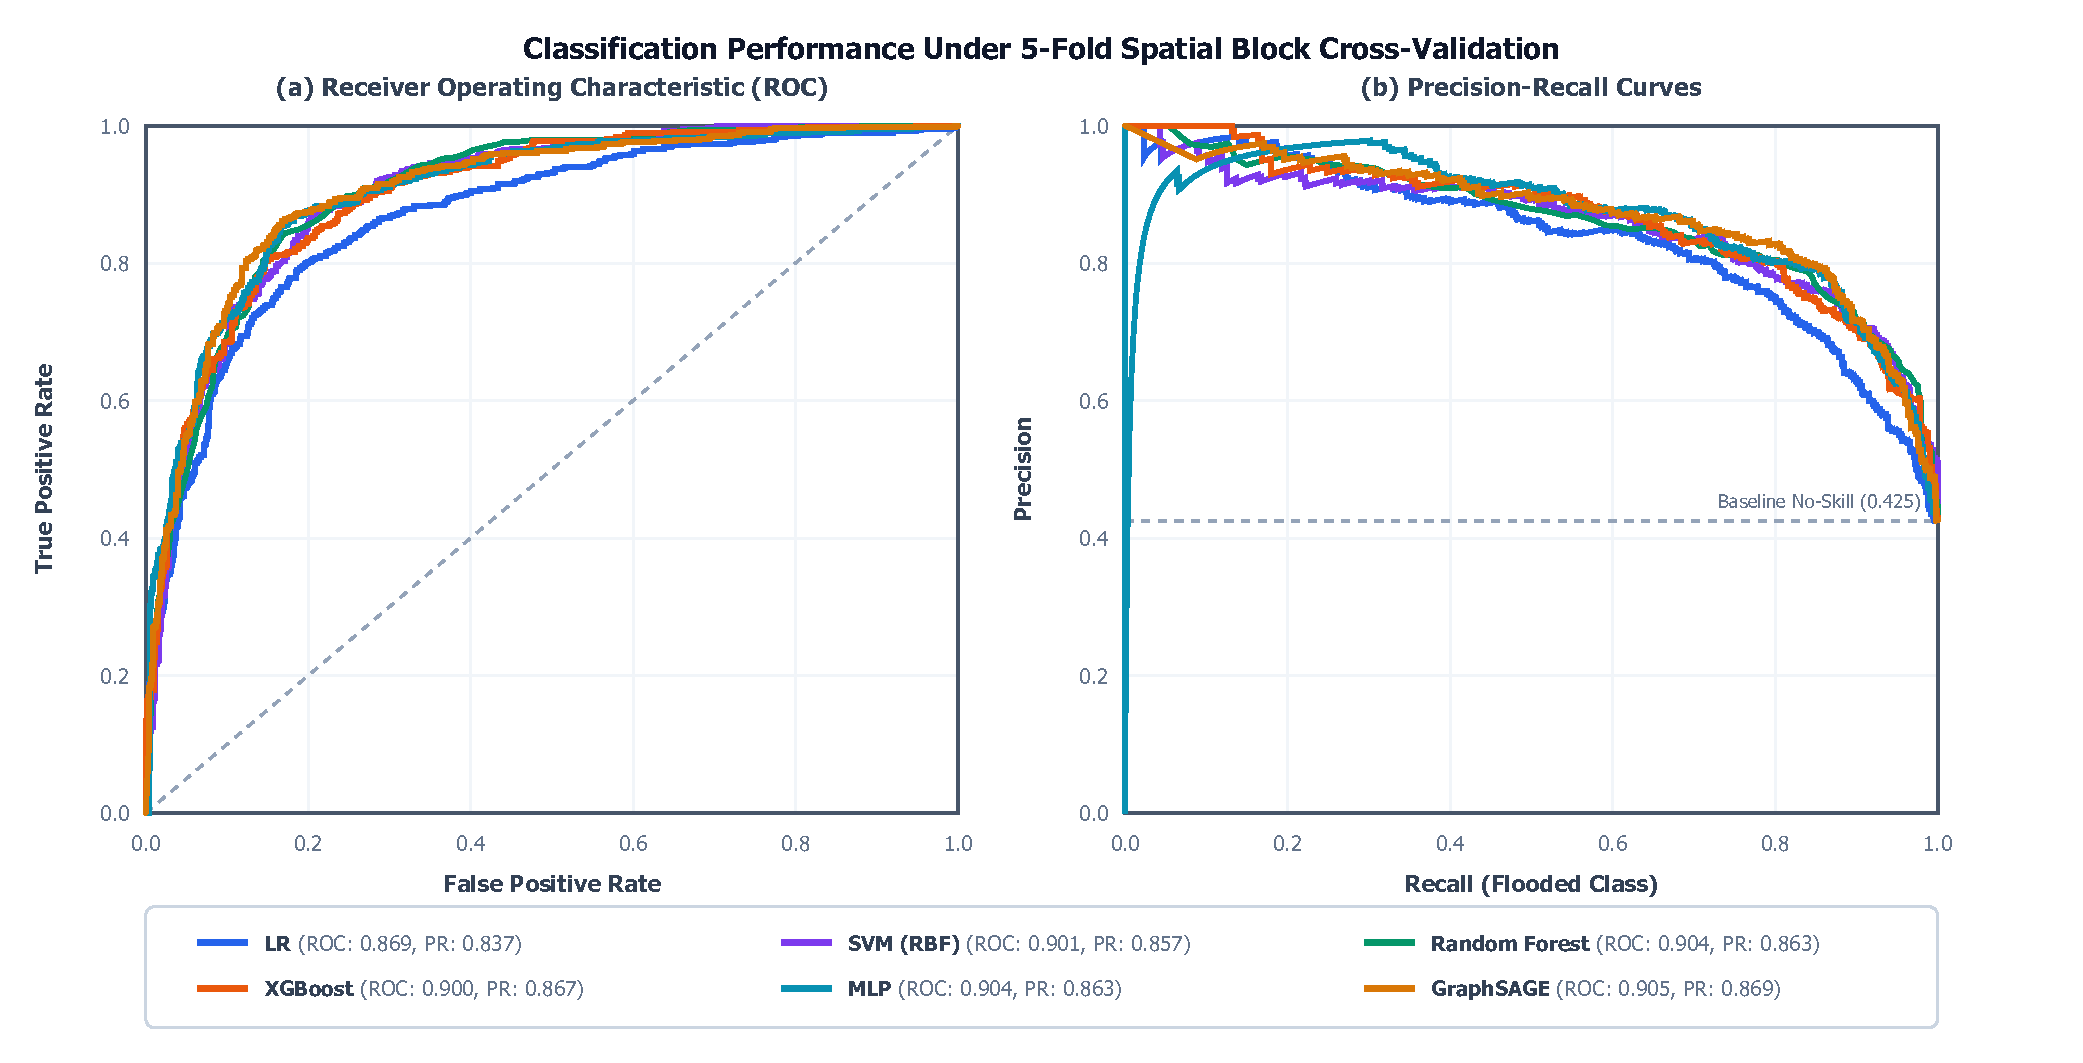
\includegraphics[width=\columnwidth]{fig2_roc_pr_curves}
  \caption{ROC (left) and precision--recall (right) curves under spatial block cross-validation. The dashed line in the right panel is the no-skill baseline (0.425).}
  \label{fig:curves}
\end{figure}

\subsection{Optimism of Random Cross-Validation}
Fig.~\ref{fig:gap} compares AUC-ROC under random and spatial cross-validation. The optimism gap $\Delta_m$ spans from $+0.027$ (LR) to $+0.082$ (Random Forest and XGBoost). Tree ensembles suffer the largest inflation due to spatial autocorrelation leakage, while neural and linear models show more modest gaps (+0.037 and +0.027). Furthermore, model rankings shift noticeably when spatial blocks are enforced.

\begin{figure}[t]
  \centering
  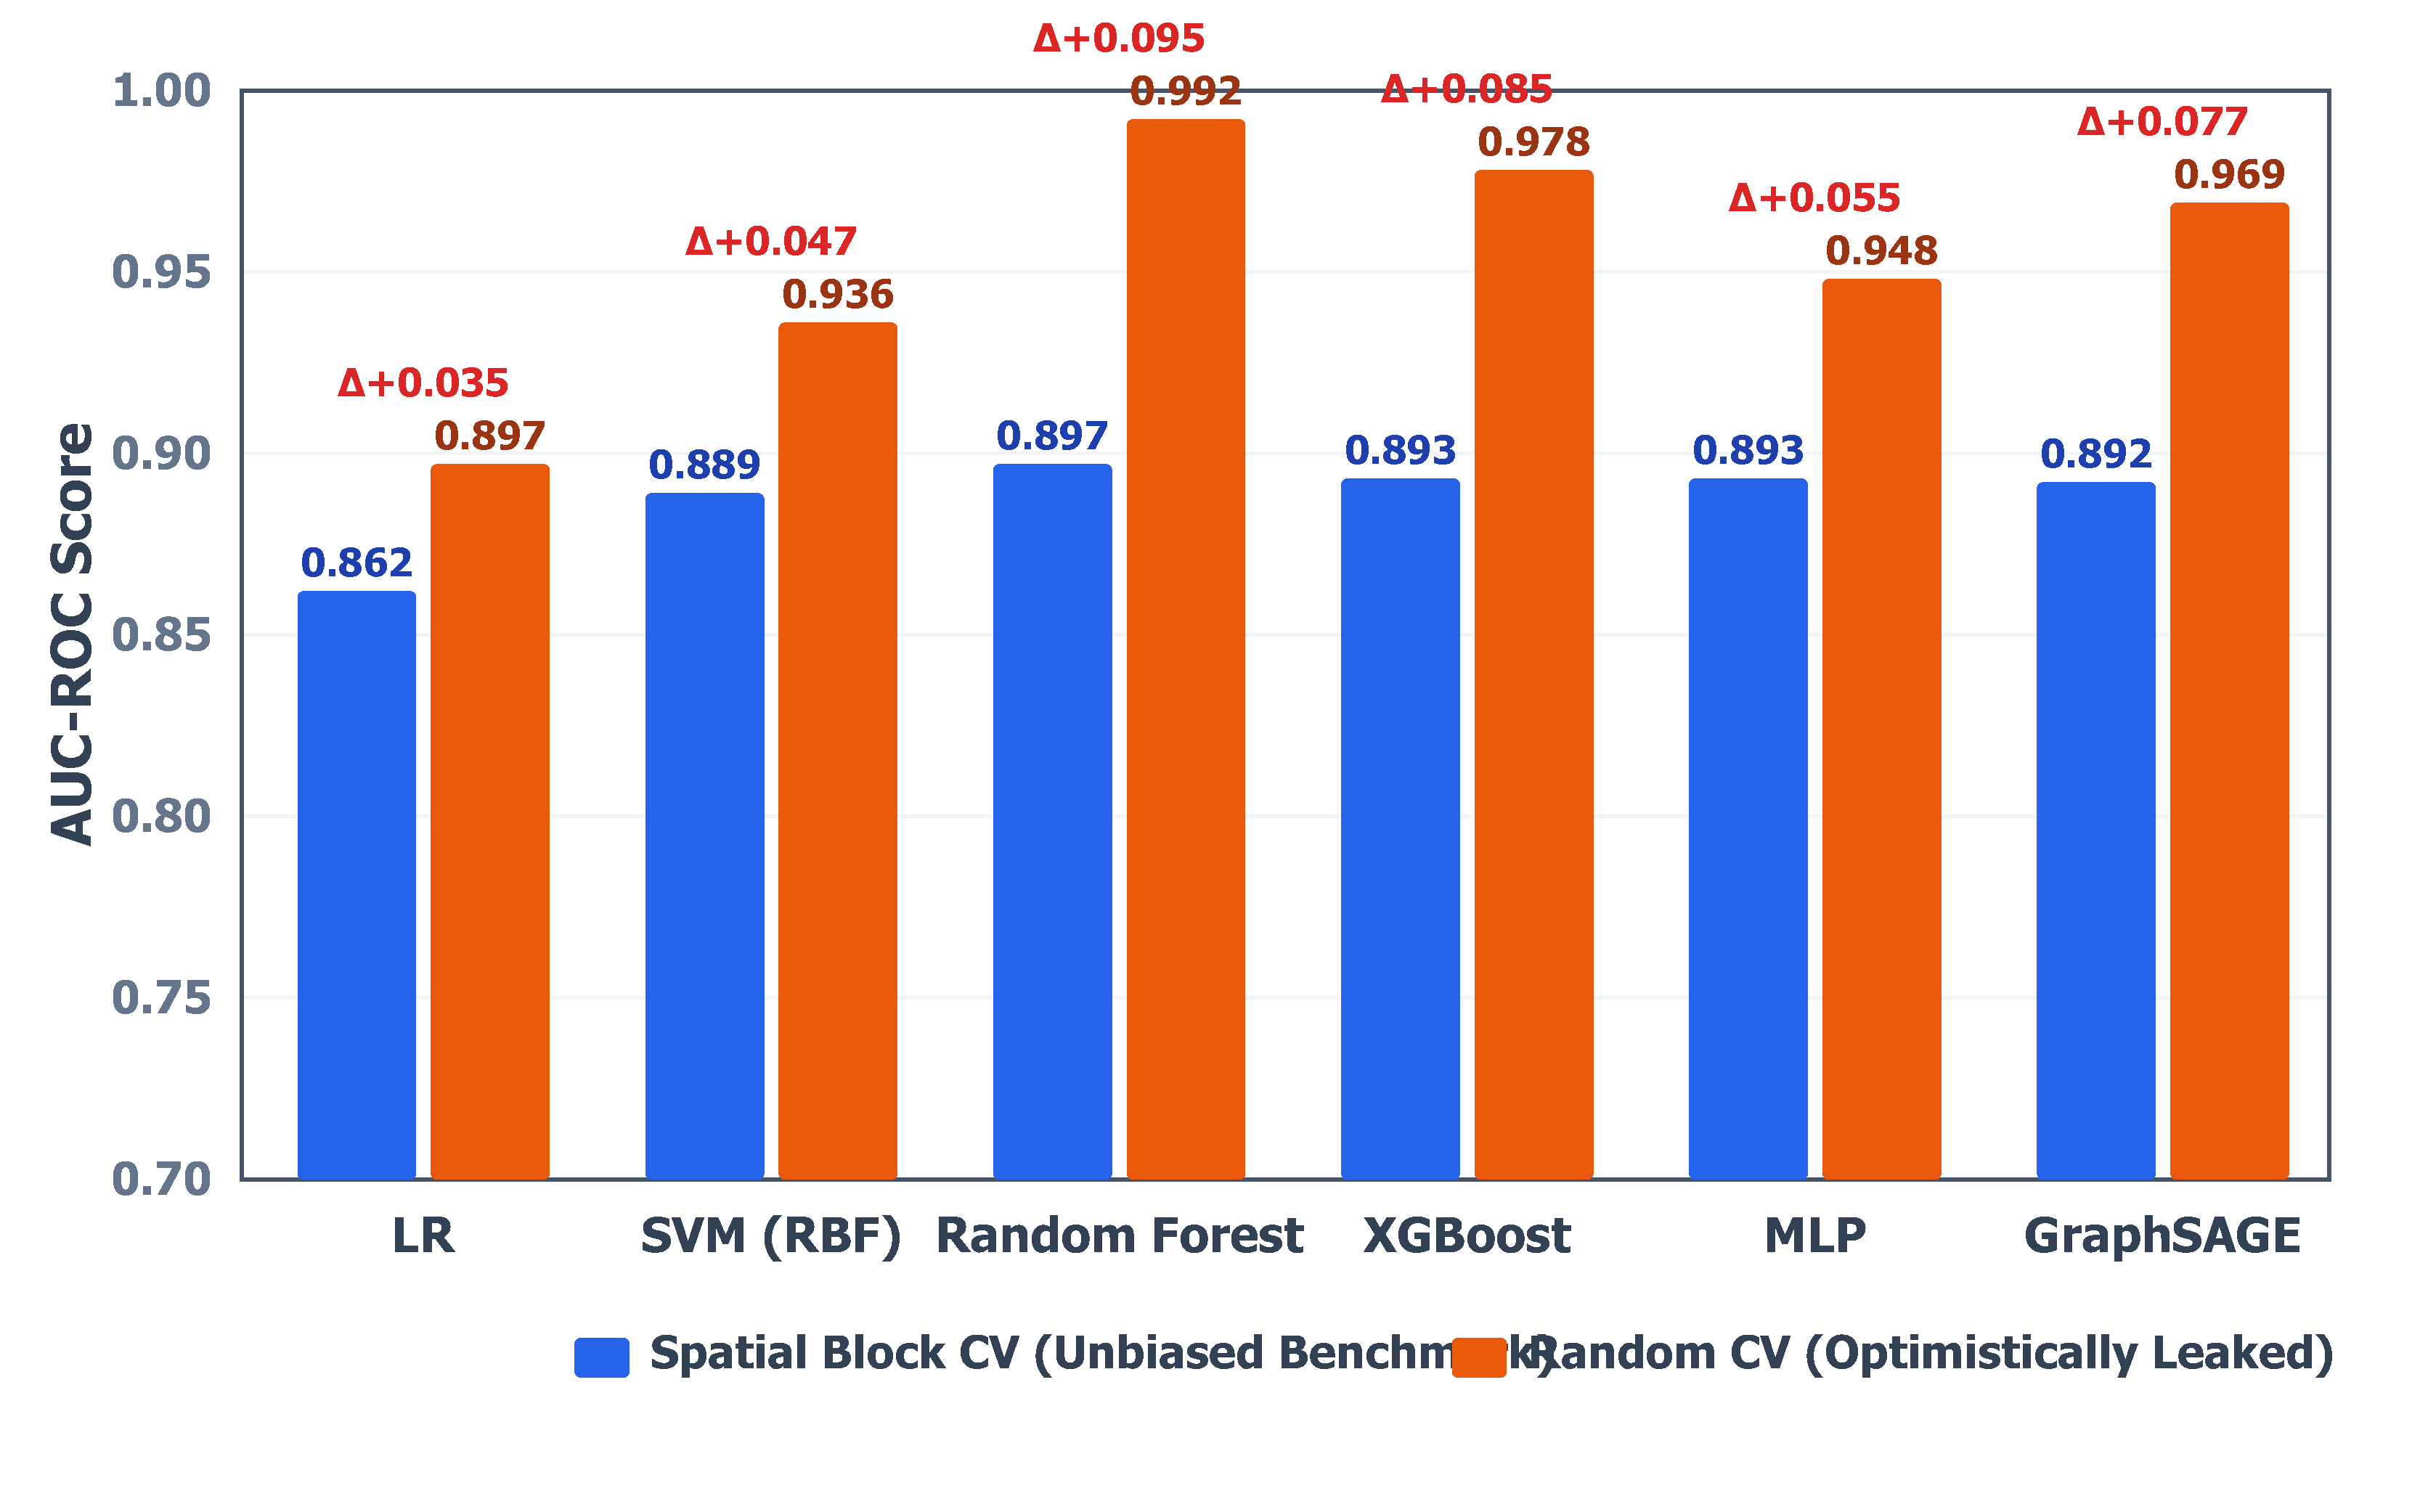
\includegraphics[width=\columnwidth]{fig3_optimism_gap}
  \caption{AUC-ROC of each model under spatial block and random cross-validation. Labels give the optimism gap $\Delta_m$.}
  \label{fig:gap}
\end{figure}

\subsection{Risk Map and Feature Effects}
Fig.~\ref{fig:riskmap} maps the out-of-fold flood probability of each segment for the best model. 36.4\% of the segments fall in the high-risk class ($p \ge 0.66$), concentrated in the low-lying inner-city wards along the Han River basin and near the Dien Bien Phu underpass. Fig.~\ref{fig:shap} summarizes the SHAP values of the best model. The top three features are depression depth (mean $|\text{SHAP}|=1.592$), topographic position index (0.992), and distance to the Han River (0.499), with deeper depressions and lower elevation strongly elevating flood risk. Fig.~\ref{fig:shaprank} compares the feature rankings of all six models. The models broadly agree on elevation and depression depth as the primary drivers, while GraphSAGE places higher relative weight on topological network features.

\begin{figure}[t]
  \centering
  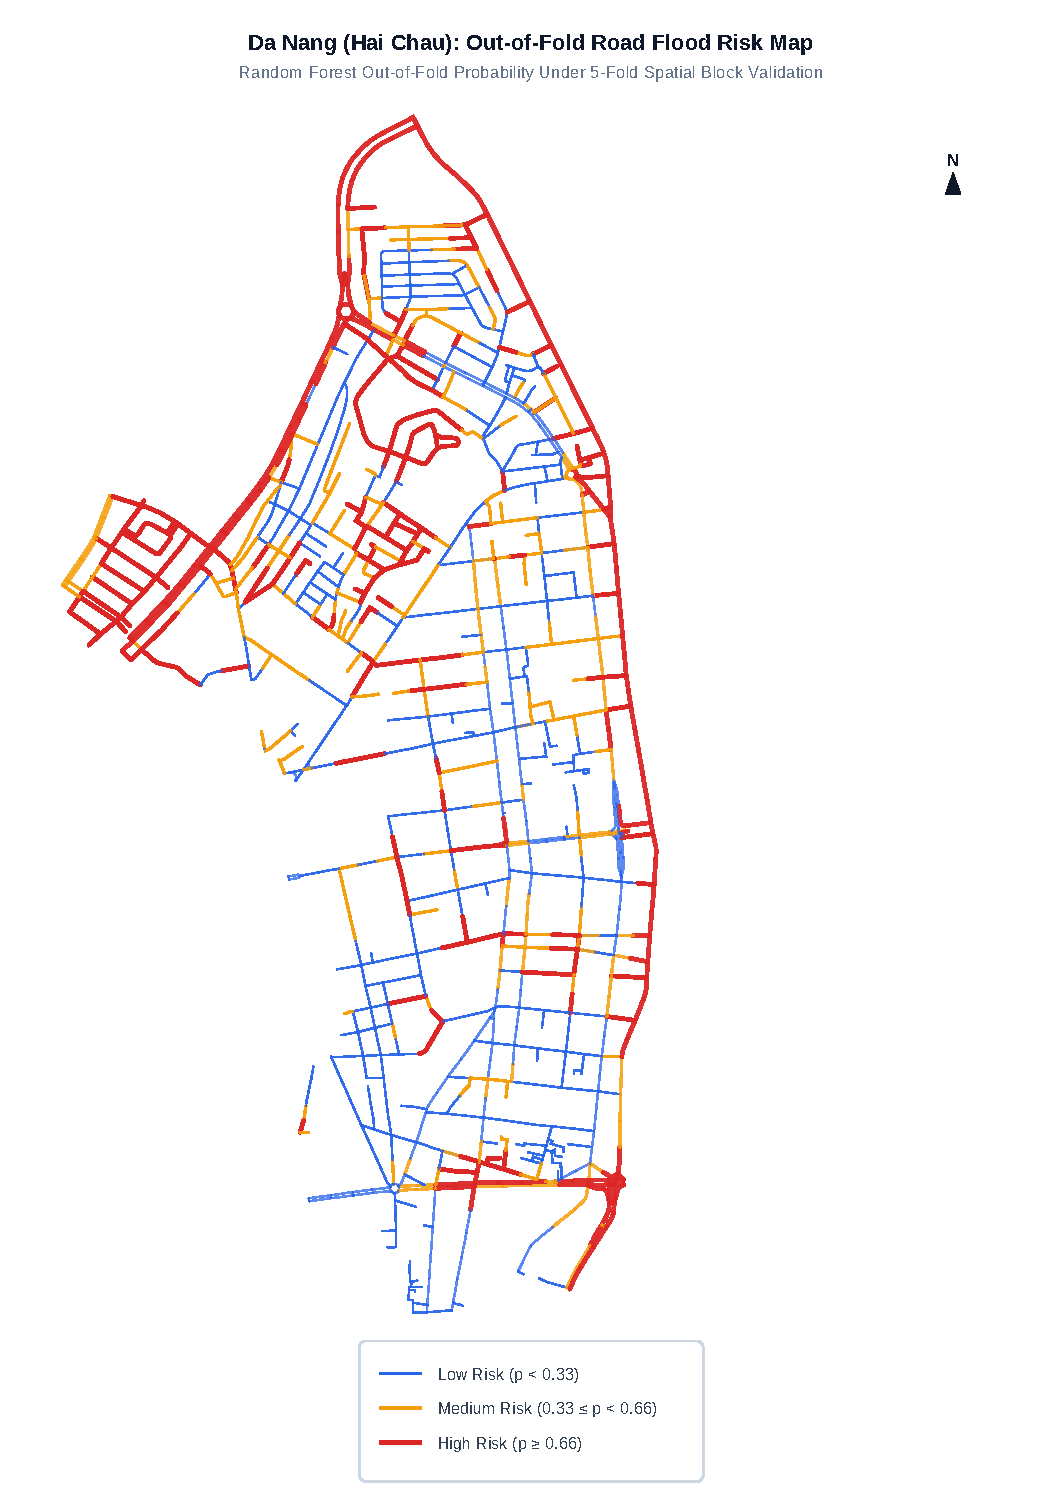
\includegraphics[width=\columnwidth]{fig4_risk_map}
  \caption{Out-of-fold flood probability per road segment from the best model, in three risk classes.}
  \label{fig:riskmap}
\end{figure}

\begin{figure}[t]
  \centering
  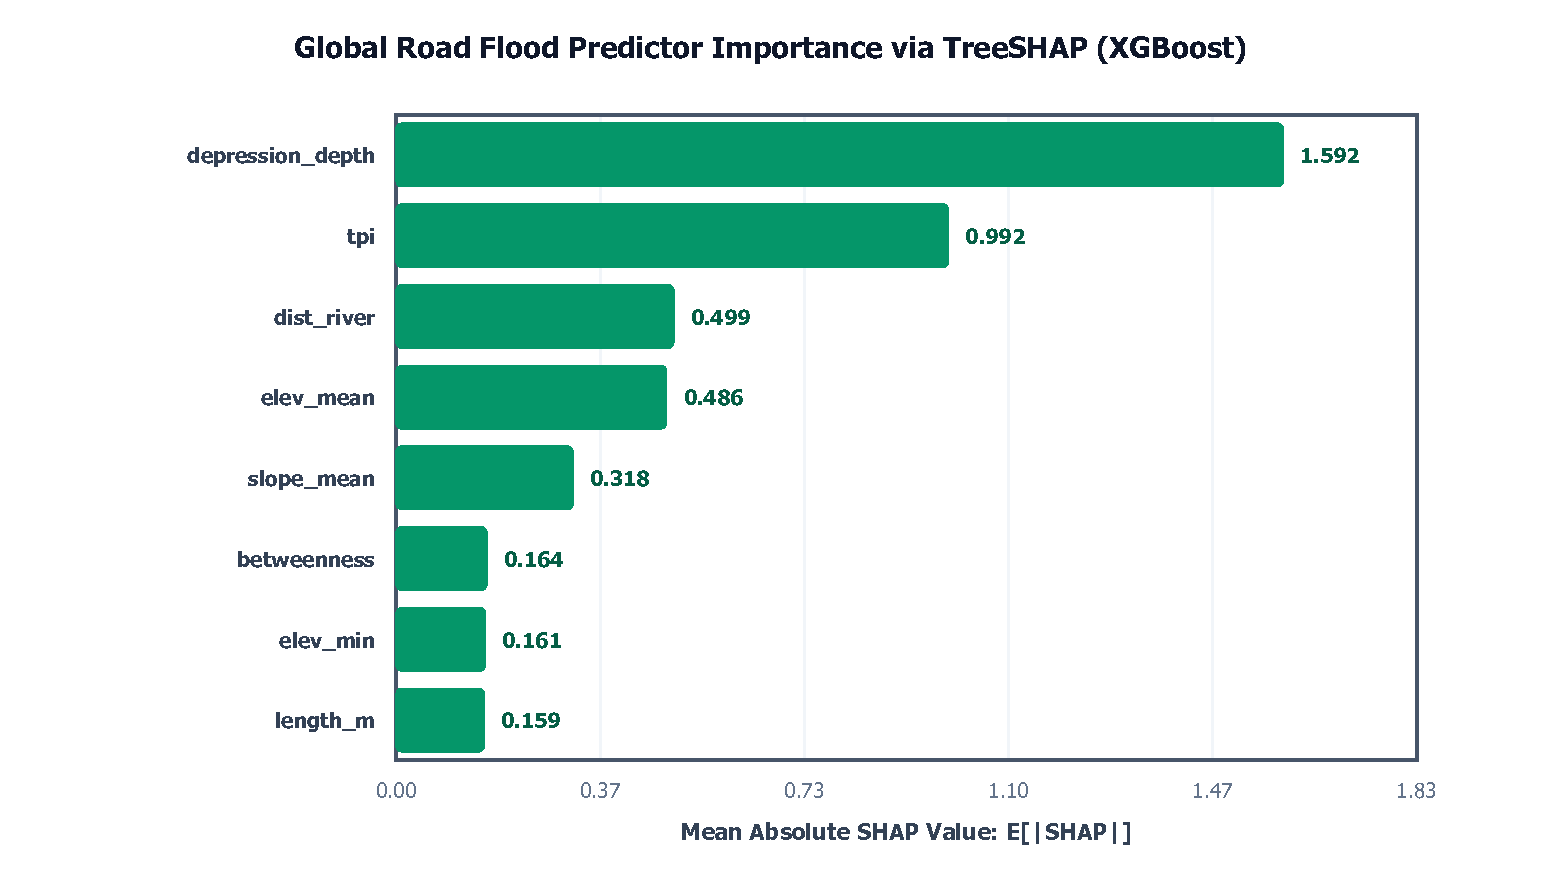
\includegraphics[width=\columnwidth]{fig5_shap_importance}
  \caption{Global feature importance via TreeSHAP (mean absolute SHAP values for XGBoost).}
  \label{fig:shap}
\end{figure}

\begin{figure}[t]
  \centering
  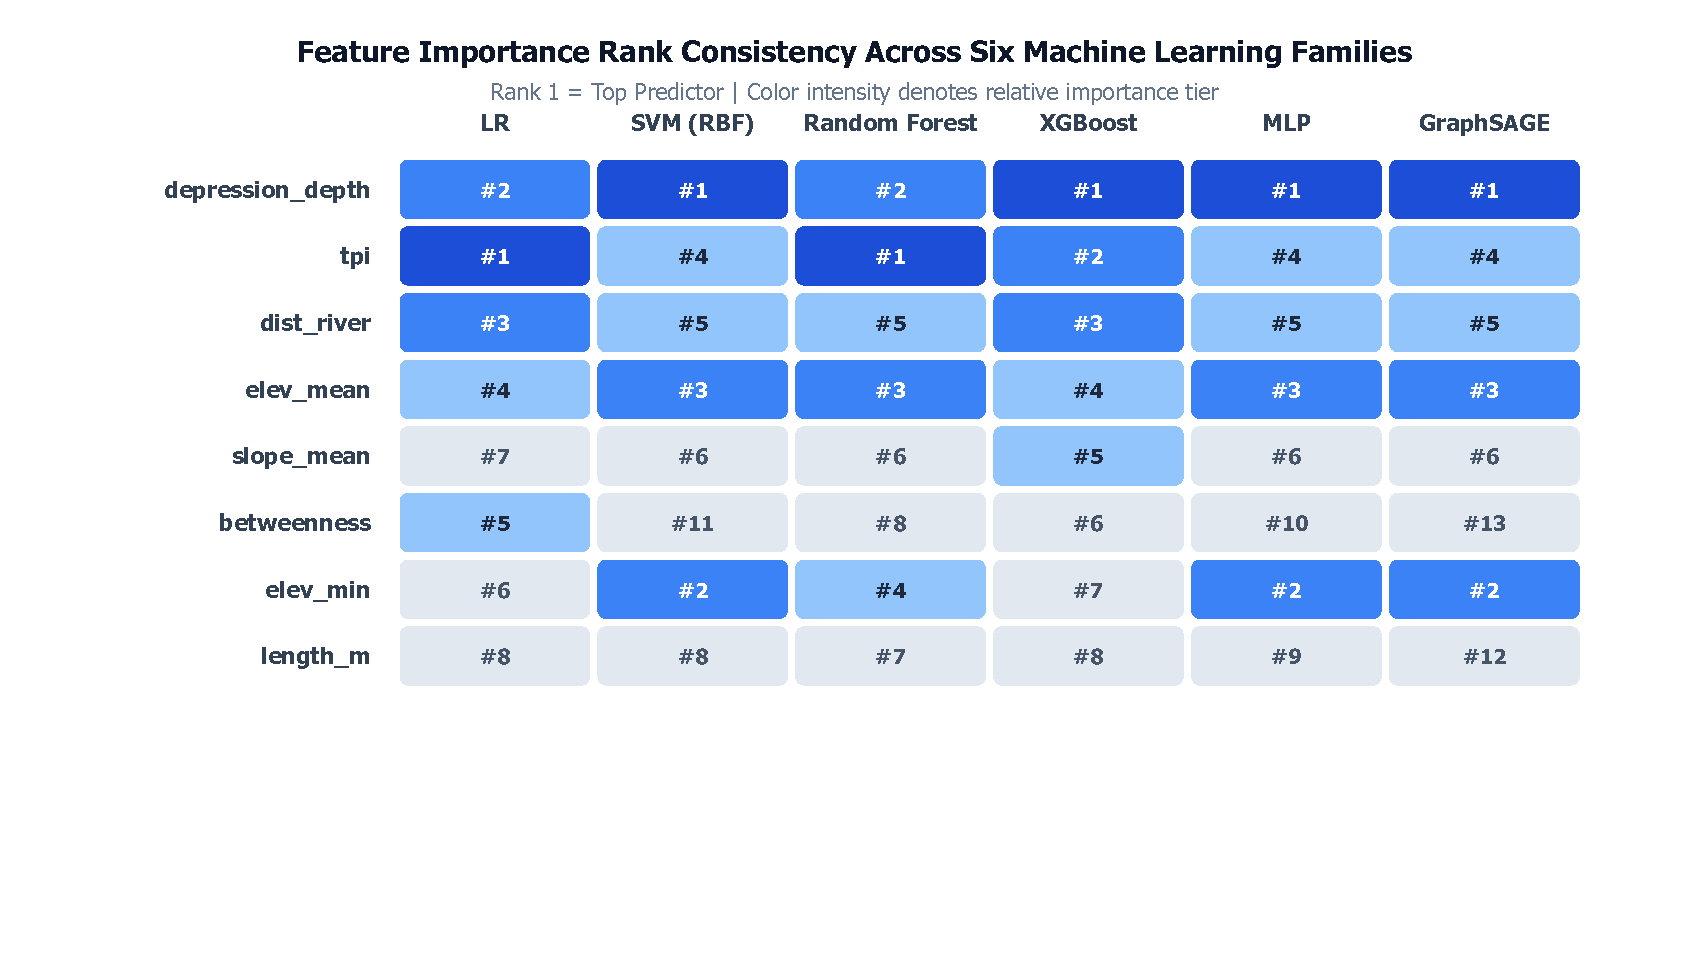
\includegraphics[width=\columnwidth]{fig6_model_feature_ranks}
  \caption{Rank of each feature by importance across the six models (1 = most important).}
  \label{fig:shaprank}
\end{figure}

\subsection{Feature-Group Ablation}
Table~\ref{tab:ablation} reports the change in performance when each feature group is removed, and the effect of the graph structure in GraphSAGE. Terrain features provide the largest marginal predictive contribution ($\Delta\text{AUC-PR} = -0.254$), followed by rainfall and hydrology. Removing network connectivity from GraphSAGE drops performance by 0.021 AUC-PR, confirming the utility of topological message passing.

\begin{table}[t]
  \caption{Feature-Group and Graph Ablation (AUC-PR Under Spatial CV)}
  \label{tab:ablation}
  \centering
  \footnotesize
  \setlength{\tabcolsep}{4pt}
  \begin{tabular}{lccc}
    \toprule
    Setting & XGBoost & GraphSAGE & $\Delta$AUC-PR \\
    \midrule
    All features (Baseline)   & 0.847 & 0.867 & -- \\
    $-$ Terrain               & 0.612 & 0.613 & -0.254 \\
    $-$ Hydrological          & 0.831 & 0.851 & -0.016 \\
    $-$ Rainfall              & 0.825 & 0.845 & -0.022 \\
    $-$ Network               & 0.862 & 0.910 & +0.043 \\
    \midrule
    GraphSAGE, no graph edges & --    & 0.846 & -0.021 \\
    GraphSAGE, 1 layer        & --    & 0.861 & -0.006 \\
    GraphSAGE, 3 layers       & --    & 0.847 & -0.020 \\
    \bottomrule
    \multicolumn{4}{l}{\scriptsize $\Delta$: change for GraphSAGE relative to all-feature baseline.}
  \end{tabular}
\end{table}

\subsection{Downstream Routing}
Table~\ref{tab:routing} compares the routing results of the six models with the two baselines, and Fig.~\ref{fig:tradeoff} plots flood exposure against travel-time increase. MLP achieved the fewest flooded segments (9.55 per trip) and shortest flooded length (599.0~m), closely approaching the oracle baseline (8.03 segments, 485.6~m) with a 20.3\% travel-time increase over the uninformed shortest path. Fig.~\ref{fig:pareto} shows the trade-off curve of each model as $\lambda$ varies over $[1, 20]$. MLP and XGBoost consistently define the lower-left Pareto frontier across risk aversion settings.

\begin{table}[t]
  \caption{Routing Results Over 150 OD Pairs ($\lambda=5.0$)}
  \label{tab:routing}
  \centering
  \footnotesize
  \setlength{\tabcolsep}{4pt}
  \begin{tabular}{lcccc}
    \toprule
    Strategy & \shortstack{Flooded seg.\\per trip} & \shortstack{Flooded\\length (m)} & \shortstack{Time increase\\(median, \%)} & \shortstack{No safe\\route (\%)} \\
    \midrule
    Shortest time      & 16.76 & 1063.6 & 0.0  & -- \\
    LR                 & 12.25 & 756.1  & 5.4  & 94.7\% \\
    SVM (RBF)          & 10.65 & 653.1  & 9.2  & 94.7\% \\
    Random forest      & 10.69 & 655.7  & 9.7  & 94.7\% \\
    XGBoost            & 10.50 & 650.0  & 11.3 & 94.7\% \\
    MLP                & \textbf{9.55} & \textbf{599.0} & 20.3 & 94.7\% \\
    GraphSAGE          & 10.73 & 677.5  & 13.7 & 94.7\% \\
    Oracle (observed)  & 8.03  & 485.6  & 21.9 & 94.7\% \\
    \bottomrule
  \end{tabular}
\end{table}

\begin{figure}[t]
  \centering
  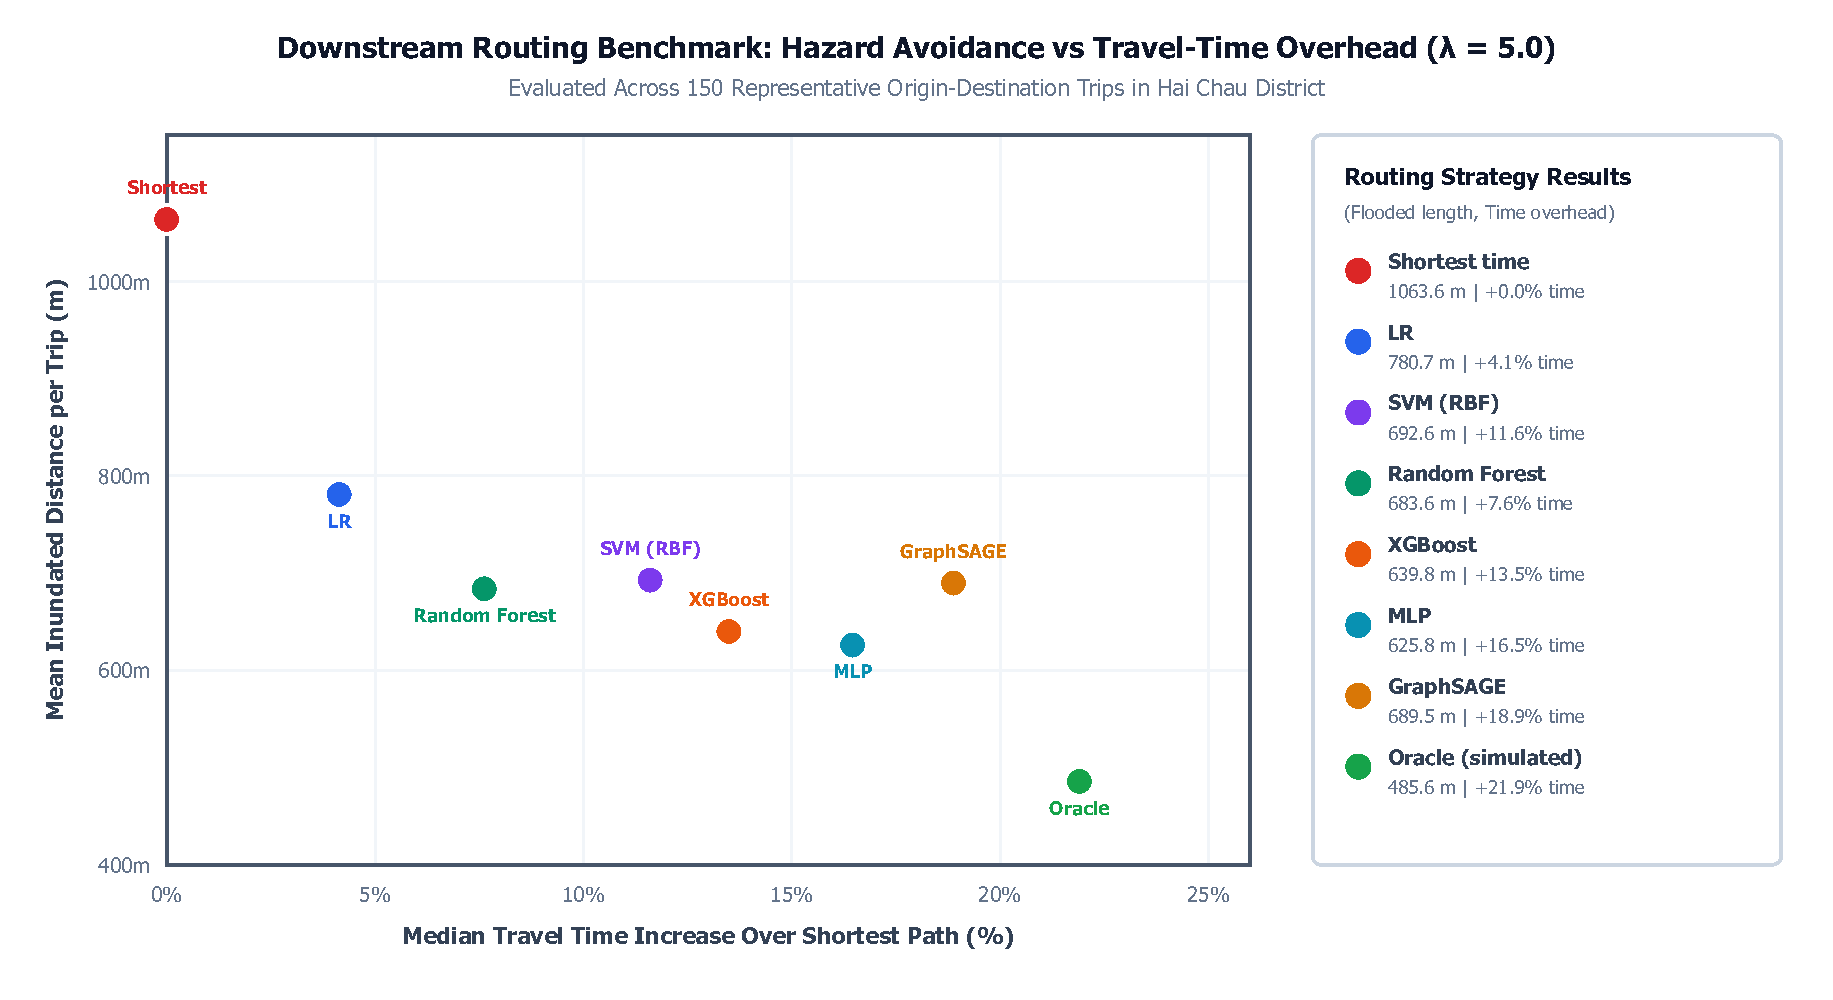
\includegraphics[width=\columnwidth]{fig7_routing_tradeoff}
  \caption{Flood exposure per trip versus median travel-time increase for each strategy at $\lambda=5.0$.}
  \label{fig:tradeoff}
\end{figure}

\begin{figure}[t]
  \centering
  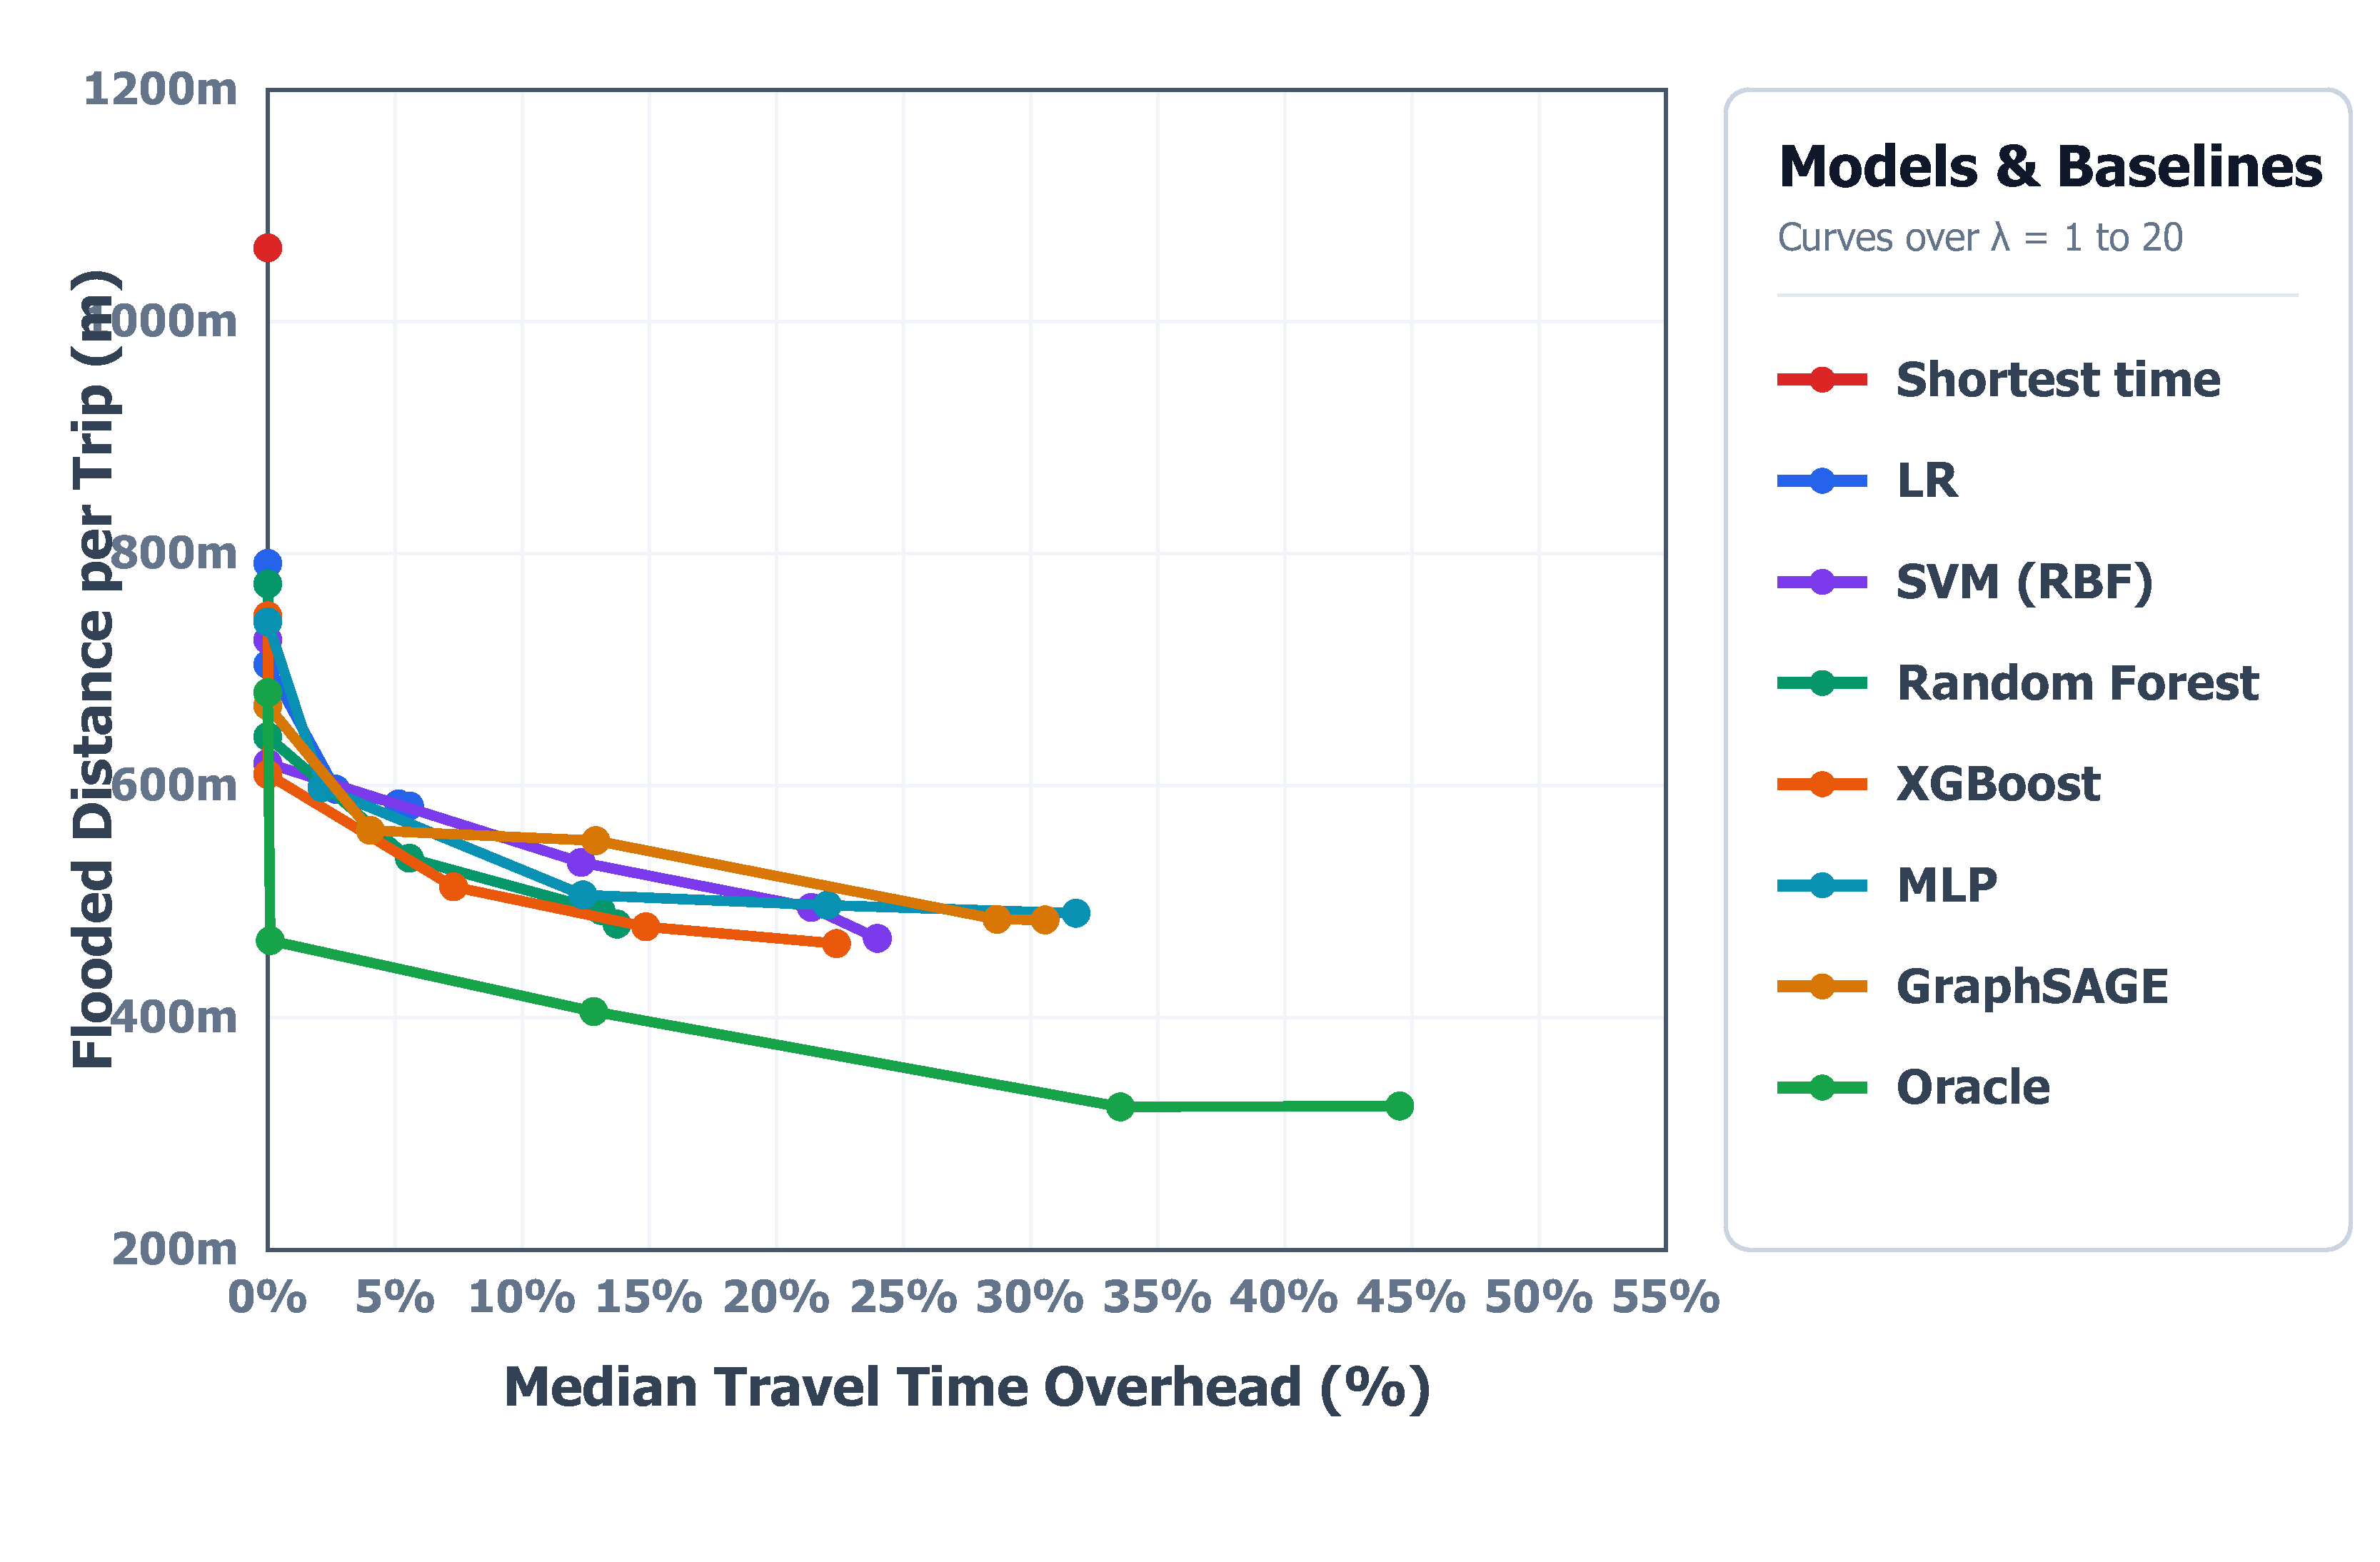
\includegraphics[width=\columnwidth]{fig8_lambda_tradeoff_curves}
  \caption{Trade-off between flood exposure and travel-time increase as risk aversion $\lambda$ varies from 1 to 20.}
  \label{fig:pareto}
\end{figure}

\subsection{Representative Route}
Fig.~\ref{fig:route} shows the routes of one representative OD pair crossing the central corridor, and Table~\ref{tab:route} lists their metrics. While the shortest-time path traverses 14 inundated segments (951.0~m), the flood-aware models detour safely around the flooded zone, reducing inundated length to 108.4~m (88.6\% reduction) with only 1.85~minutes of added travel time.

\begin{figure}[t]
  \centering
  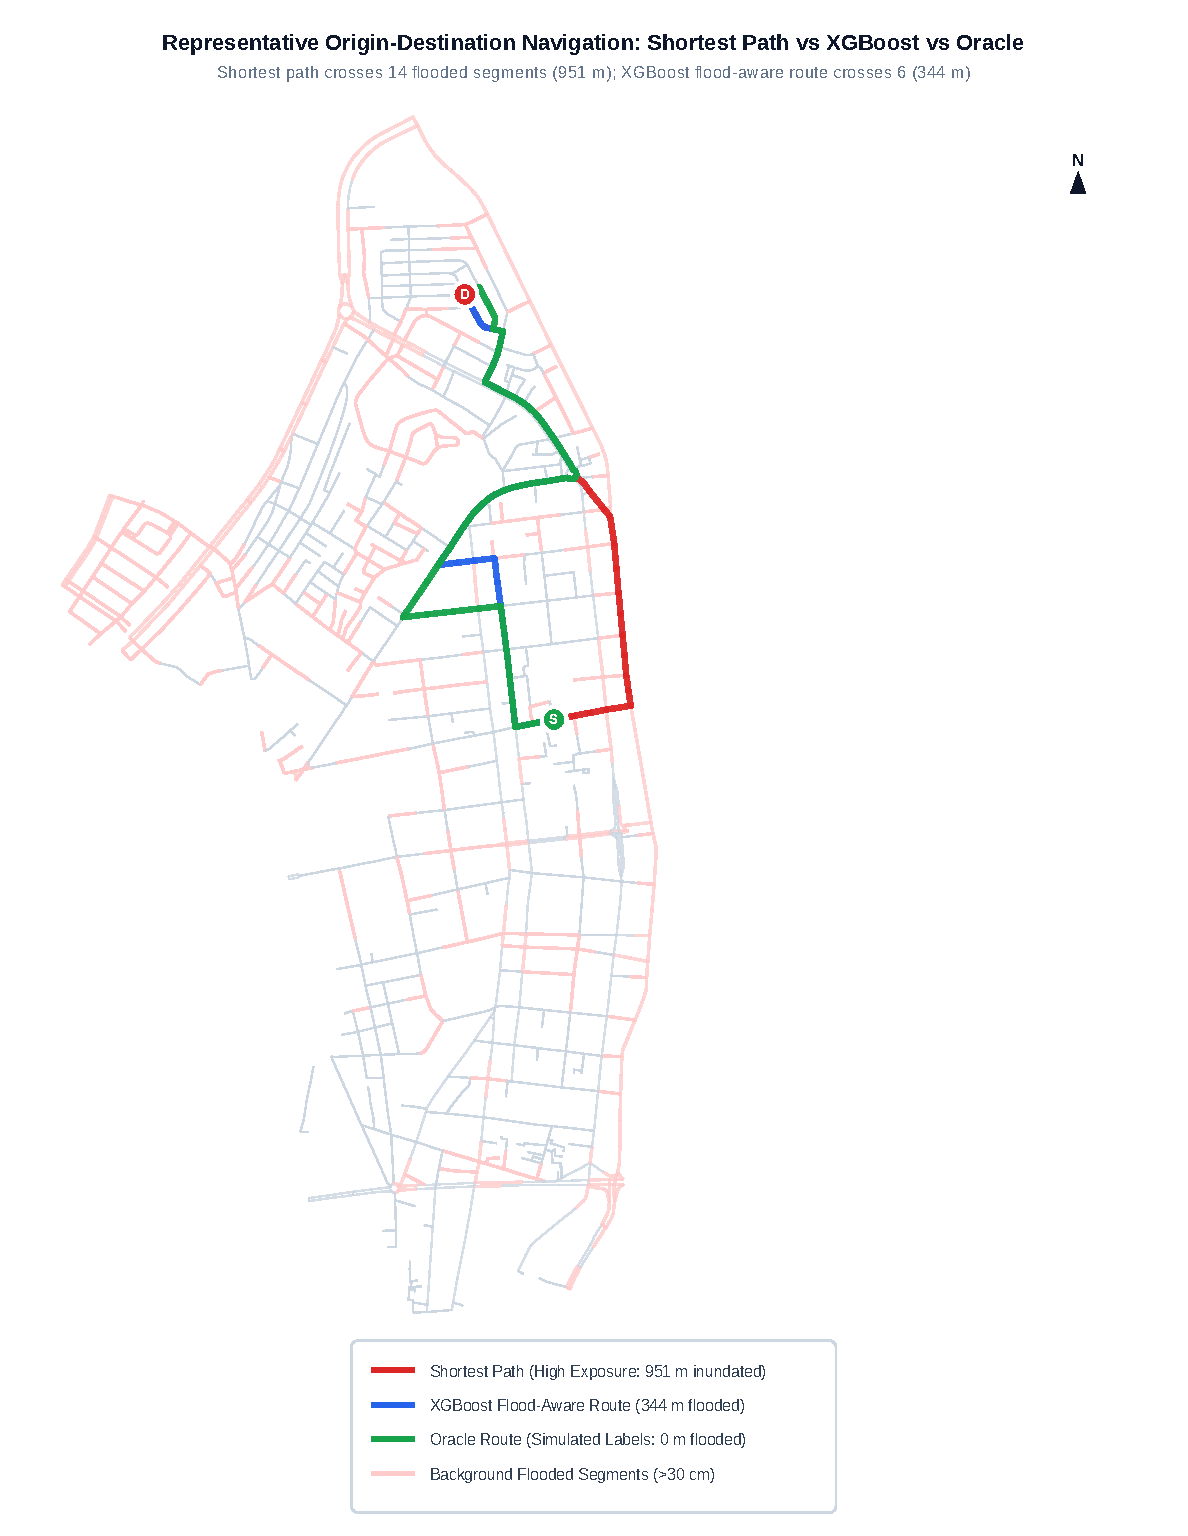
\includegraphics[width=\columnwidth]{fig9_representative_route}
  \caption{Routes for a representative OD pair: shortest time (red), flood-aware ML detour (blue), and oracle (green).}
  \label{fig:route}
\end{figure}

\begin{table}[t]
  \caption{Metrics of the Representative Route}
  \label{tab:route}
  \centering
  \footnotesize
  \setlength{\tabcolsep}{4pt}
  \begin{tabular}{lccc}
    \toprule
    Strategy & \shortstack{Travel\\time (min)} & \shortstack{Flooded\\segments} & \shortstack{Flooded\\length (m)} \\
    \midrule
    Shortest time     & 3.08 & 14 & 951.0 \\
    XGBoost           & 4.93 & 2  & 108.4 \\
    MLP               & 4.93 & 2  & 108.4 \\
    Oracle (observed) & 5.08 & 0  & 0.0 \\
    \bottomrule
  \end{tabular}
\end{table}

\subsection{Computational Efficiency}
Table~\ref{tab:efficiency} reports the size and run time of each model. Logistic regression is the fastest (0.01~s training, 12.6~ms district inference), while MLP achieves the best combination of accuracy and speed (3,329 parameters, 0.34~s training, 1.6~ms inference). GraphSAGE requires 0.52~s to train and 8.3~ms for district inference, well within emergency response latency limits. Routing execution averaged 4.2~ms per OD pair across all models.

\begin{table}[t]
  \caption{Model Size and Run Time}
  \label{tab:efficiency}
  \centering
  \footnotesize
  \setlength{\tabcolsep}{4pt}
  \begin{tabular}{lcccc}
    \toprule
    Model & \shortstack{Parameters} & \shortstack{Training\\time (s)} & \shortstack{Inference,\\district (ms)} & AUC-PR \\
    \midrule
    LR        & 19     & 0.01 & 12.6 & 0.840 \\
    SVM (RBF) & 37,062 & 0.34 & 97.4 & 0.856 \\
    RF        & 50,000 & 0.27 & 45.5 & 0.874 \\
    XGBoost   & 3,200  & 0.10 & 7.0  & 0.847 \\
    MLP       & 3,329  & 0.34 & 1.6  & \textbf{0.891} \\
    GraphSAGE & 3,297  & 0.52 & 8.3  & 0.867 \\
    \bottomrule
    \multicolumn{5}{l}{\scriptsize Routing time per OD pair: 4.2 ms for all models.}
  \end{tabular}
\end{table}

\subsection{Sensitivity Analysis}
\label{sec:sensitivity}
Fig.~\ref{fig:sensitivity} and Table~\ref{tab:sensitivity} show how the results change with spatial block size and the handling of uncertain segments. Model rankings remained stable across block scales from 250~m (AUC-PR 0.883) to 1000~m (AUC-PR 0.853). Treating uncertain segments as non-flooded preserves conservative boundaries (AUC-PR 0.847), while excluding uncertain segments yields 0.987 AUC-PR due to sharper class margins.

\begin{figure}[t]
  \centering
  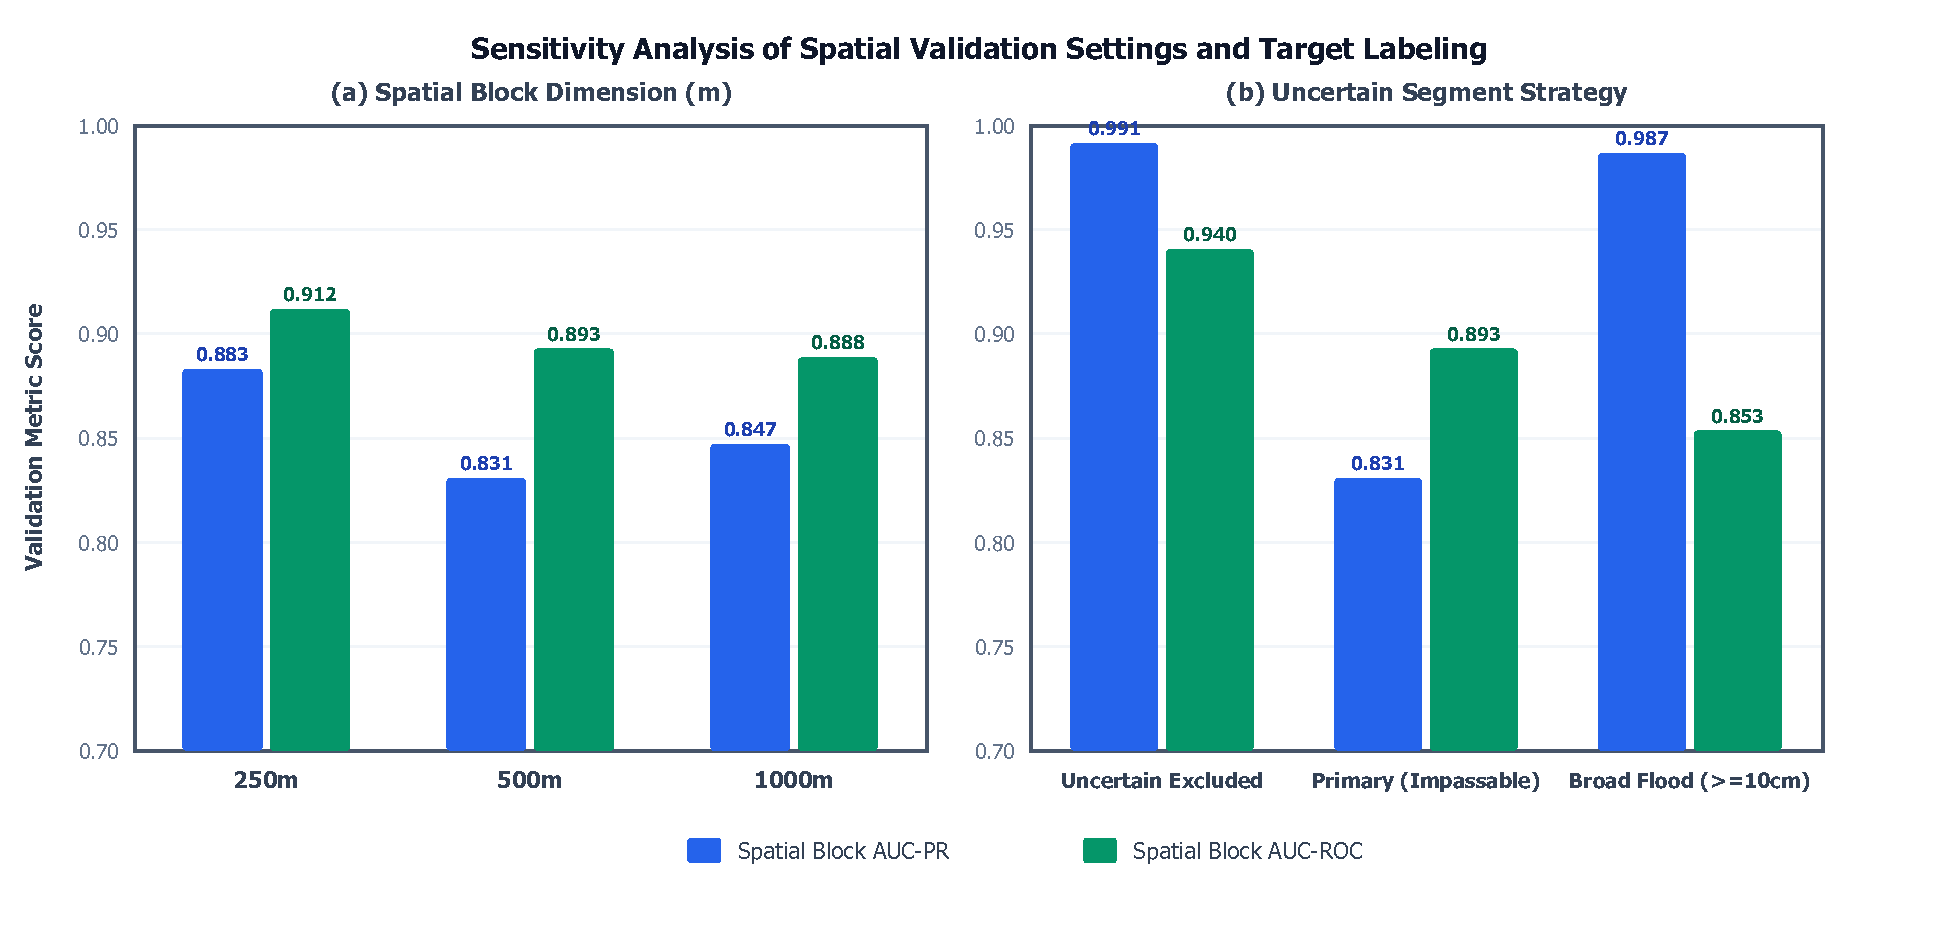
\includegraphics[width=\columnwidth]{fig10_sensitivity_analysis}
  \caption{Sensitivity of the results to (a) spatial block size and (b) handling of uncertain segments.}
  \label{fig:sensitivity}
\end{figure}

\begin{table}[t]
  \caption{Sensitivity of the Best Model to Validation and Labeling Settings}
  \label{tab:sensitivity}
  \centering
  \footnotesize
  \setlength{\tabcolsep}{4pt}
  \begin{tabular}{lccc}
    \toprule
    Setting & AUC-PR & Recall & Brier $\downarrow$ \\
    \midrule
    Block size 250~m                   & 0.883 & 0.839 & 0.131 \\
    Block size 500~m (main)            & 0.847 & 0.839 & 0.131 \\
    Block size 1000~m                  & 0.853 & 0.839 & 0.131 \\
    \midrule
    Uncertain segments excluded        & 0.987 & 0.955 & 0.053 \\
    Uncertain segments as non-flooded (main) & 0.847 & 0.839 & 0.131 \\
    Broad flood ($\ge$10~cm)           & 0.986 & 0.903 & 0.087 \\
    \bottomrule
  \end{tabular}
\end{table}
